% Created 2019-02-04 Mon 14:03
\documentclass[11pt]{article}
\usepackage[utf8]{inputenc}
\usepackage[T1]{fontenc}
\usepackage{fixltx2e}
\usepackage{graphicx}
\usepackage{grffile}
\usepackage{longtable}
\usepackage{wrapfig}
\usepackage{rotating}
\usepackage[normalem]{ulem}
\usepackage{amsmath}
\usepackage{textcomp}
\usepackage{amssymb}
\usepackage{capt-of}
\usepackage{hyperref}
\usepackage{amsmath}
\usepackage{amssymb}
\author{Jack Truskowski}
\date{\today}
\title{CS744: Big Data Systems}
\hypersetup{
 pdfauthor={Jack Truskowski},
 pdftitle={CS744: Big Data Systems},
 pdfkeywords={},
 pdfsubject={},
 pdfcreator={Emacs 25.2.2 (Org mode 8.3.5)}, 
 pdflang={English}}
\begin{document}

\maketitle
\tableofcontents


\section{2/4/19 MapReduce}
\label{sec:orgheadline4}
\begin{itemize}
\item Programming model
\item Execution
\item Runtime issues
\item M-R library handles execution and run-time issues
\begin{itemize}
\item Transparent to programmers
\end{itemize}
\end{itemize}

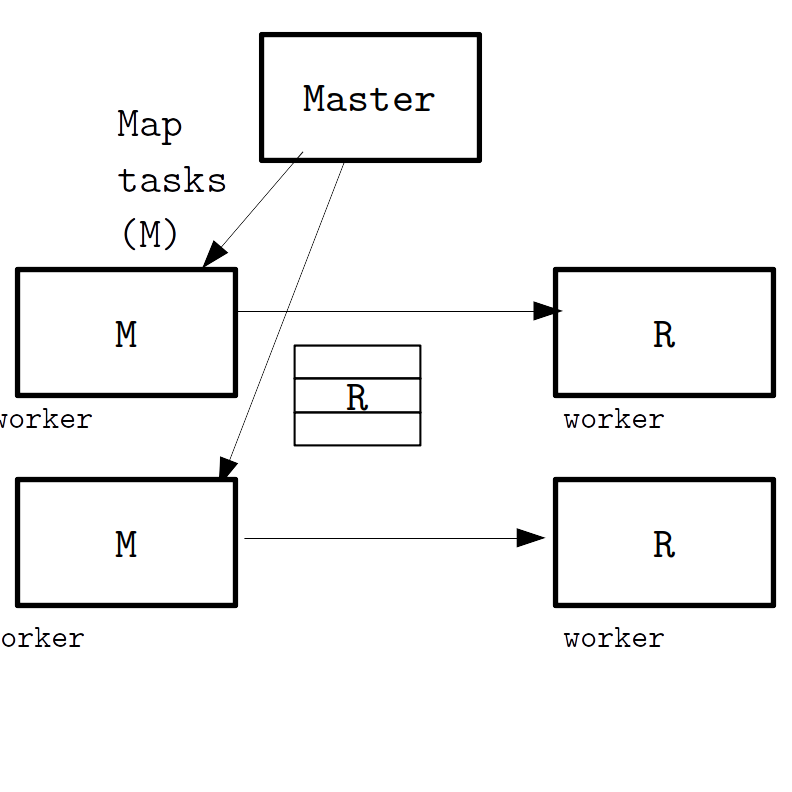
\includegraphics[width=.9\linewidth]{diagrams/masterworker.png}

\subsection{Operators}
\label{sec:orgheadline1}
\begin{enumerate}
\item Map
\begin{itemize}
\item Input = (key,value) --> (key, <v>)
\end{itemize}
\item Reduce
\begin{itemize}
\item Operates share a key
\item (key,value) is sorted and values passed to reducer
\end{itemize}
\end{enumerate}

\subsection{Failures and Slowdowns}
\label{sec:orgheadline3}
\begin{itemize}
\item Handled by the master
\end{itemize}
\subsubsection{Possible failures}
\label{sec:orgheadline2}
\begin{enumerate}
\item Map / Reduce
\begin{itemize}
\item Worker fails, some maps and some reduces completed
\item Reduce data is already written to HDFS, doesn't need to be recomputed
\item Maps must be re-executed, since it hasn't been written to HDFS
\end{itemize}
\end{enumerate}
\end{document}
